\section{Finding Crunch Spots}

\begin{wrapfigure}{l}{0.25\textwidth}
  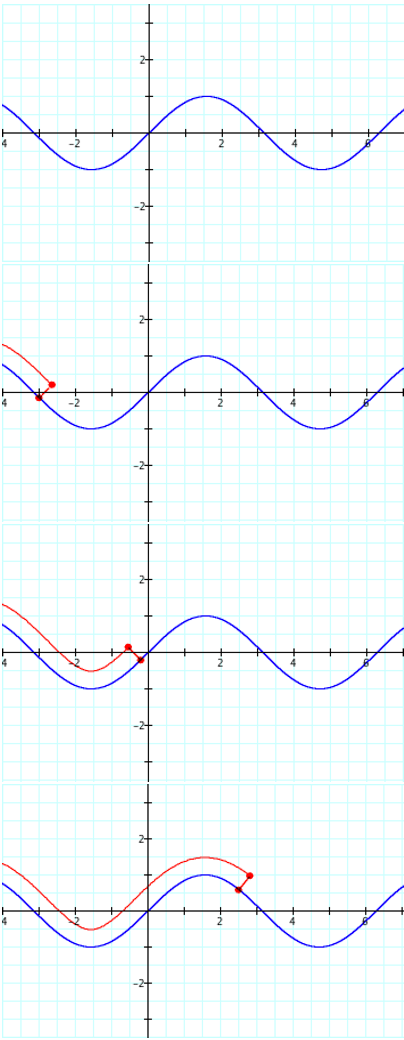
\includegraphics[width=.9\linewidth]{findig-crunch-spots-img/Fig 17.png}
  \caption{Caption}
  \label{fig:fig17}
\end{wrapfigure}

Let’s do a math thought experiment! We’re going to build a little imaginary railroad track. Imagine now that you’re standing in the Nevada desert and you wish to lay down a railroad track. Take your favorite continuously differentiable function $f(x)$. Pick a spot on the dirt to be the origin. Let the $x$-axis be East-to-West and let the $y$-axis be North-to-South. Now plot your function $f(x)$ across the desert sands using metal to form one of the railroad track rails. For the sake of
conversation let’s call it the right rail. Place a little sliding metal bit onto the track that we can push back and forth along the rail. Connect to it a metal bar of some set fixed length N that will at all times be perpendicular to the rail. Fix to the end of the metal bar a jumbo sized red magic marker that will draw upon the sand as the sliding metal bit moves along $f(x)$. As the sliding metal bit is pushed along f(x), the bar and marker will draw the left rail, aka the $N$-Units Away Curve. This set up is diagrammed in figure $\ref{fig:fig17}$. In this diagram we used $f(x) = sin(x)$.

Now add one more element to the scenario. Place onto the end of the metal beam a cool little LED light that will project a green circle of radius $N$ onto the desert sand. It ``rolls along'' the original function a little like a marble. This is diagrammed in figures $\ref{fig:fig18}$ and $\ref{fig:fig19}$. We see that this green marble rolls smoothly along the $y=f(x)$ function with its center moving precisely along the $N$-Units Away Curve. We see that for
small values of $N$ (fig $\ref{fig:fig18}$), the green marble does not intersect the original function $y=f(x)$ at all. We see that it does intersect the original function for higher $N$ values (fig $\ref{fig:fig19}$).

Now let us leave behind the Nevada desert and simply roll marbles down some functions! Let’s take the example of $y=x^2$. Take a fairly sizable marble, perhaps one of radius 2 and roll it down the curve! The following occurs:

We see that the marble gets stuck at the bottom of the parabola and cannot continue following the path of the $N$-Units Away Curve. The curve of the function got ``too tight'' for the marble to fit into. Thus we see there is correlation between the crunch spots of the $N$-Units Away Curves and portions of the original function that have maximum curvature. How can we express this connection with mathematical rigor? Luckily for us, there is already a concept of ``curvature'' in Calculus. 

To quote the classic James Stewart \textit{Calculus} textbook, ``the curvature of a function at a given point is a measure of how quickly the curve changes direction at that point'' (863.) If a tiny car were to drive along the path of the function, the curvature at a given value of $x$ gives a measure of how significantly the steering wheel of the tiny car is turned. It has formula $\kappa (x) = \dfrac{|f''(x)|}{[1 + (f'(x))^2]^{3/2}}$.

\begin{figure}[h!] 
  \label{crunch-1} 
  \begin{minipage}[b]{0.3\linewidth}
    \centering
    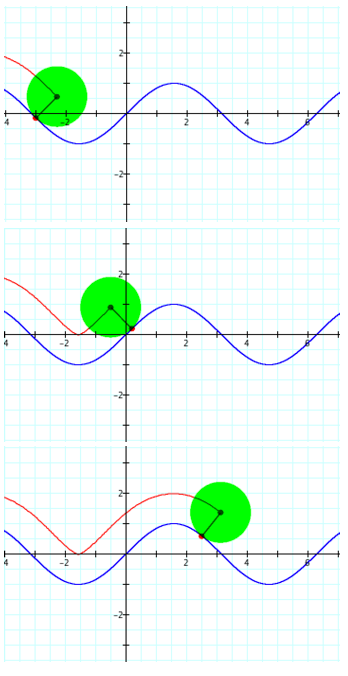
\includegraphics[width=0.9\textwidth, height=0.9\textheight, keepaspectratio]{findig-crunch-spots-img/Fig 18.png}
    \caption{Caption}
    \label{fig:fig18}
    \vspace{4ex}
  \end{minipage} % end 
  \begin{minipage}[b]{0.3\linewidth}
    \centering
    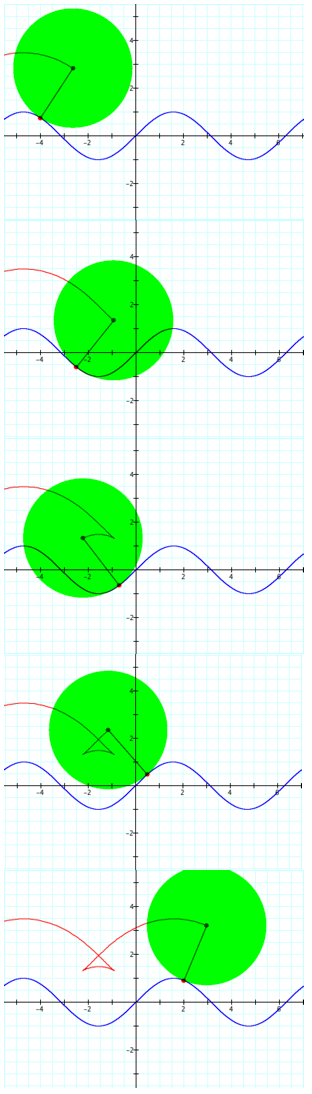
\includegraphics[width=0.9\textwidth, height=0.5\textheight, keepaspectratio]{findig-crunch-spots-img/Fig 19.png}
    \caption{Caption}
    \label{fig:fig19}
    \vspace{4ex}
  \end{minipage} % end
    \begin{minipage}[b]{0.3\linewidth}
    \centering
    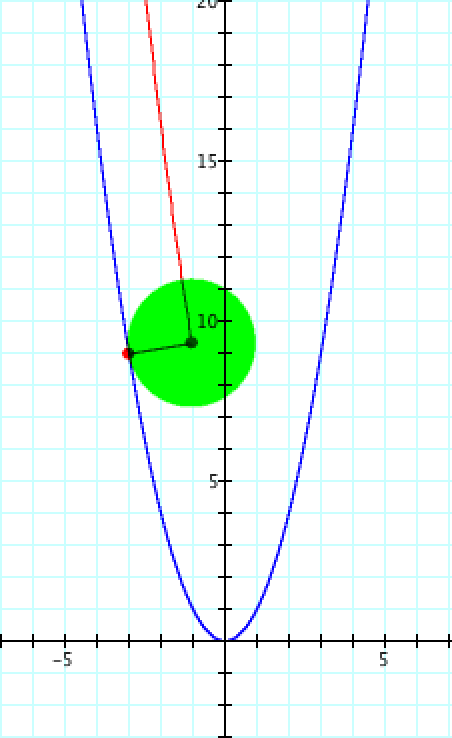
\includegraphics[width=0.9\textwidth, height=0.9\textheight, keepaspectratio]{findig-crunch-spots-img/Fig 20.png}
    \caption{Caption}
    \label{fig:fig20}
    \vspace{4ex}
  \end{minipage} % end
\end{figure}

Let’s plot the graph of a function and its curvature. (Fig $\ref{fig:fig21}$) The function will be dark blue and the curvature turquoise. If you take the multiplicative inverse of the curvature, $\dfrac{1}{\kappa (x)}$, you obtain a concept from differential geometry called the ``radius of curvature.'' We denote it by $R(x)$. It’s another way to measure how quickly the function is turning. It is equal to the radius of the circular arc which best approximates the curve at that point. (Fig $\ref{fig:fig22}$) displays $y = x^2$ next to the graph of its radius of curvature, shown in green. For an example of radius of curvature in action, here is a look at a series of points on $y = x^2$ and their ``best approximating circles'' (Fig \ref{fig:fig23}).

Let’s go on another little thought experiment. Suppose you want to roll a marble of positive radius $N$ along the function $y = f(x)$. You’re going to roll it smoothly along the curve, making sure it contacts the function at every $x$ value. What does it mean mathematically to find a spot where the marble gets ``stuck'' as in the rightmost image of (Fig $\ref{fig:fig24}$)? 

\begin{figure}[h!]
  \begin{minipage}[b]{0.5\linewidth}
    \centering
    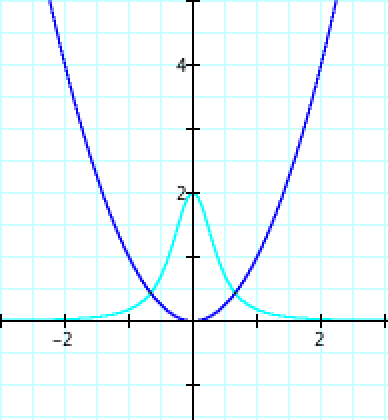
\includegraphics[width=.9\linewidth, height=0.2\textheight, keepaspectratio]{findig-crunch-spots-img/Fig 21.png}
    \caption{Caption}
    \label{fig:fig21}
    % \vspace{4ex}
  \end{minipage} % end 
  \begin{minipage}[b]{0.5\linewidth}
    \centering
    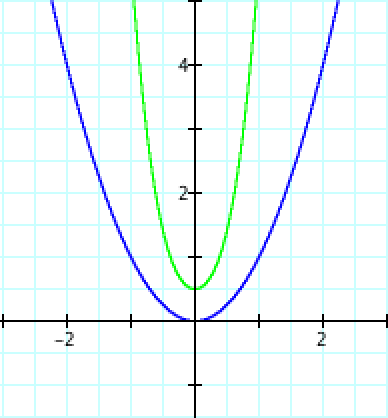
\includegraphics[width=.9\linewidth, height=0.2\textheight, keepaspectratio]{findig-crunch-spots-img/Fig 22.png}
    \caption{Caption}
    \label{fig:fig22}
    % \vspace{4ex}
  \end{minipage} % end
\end{figure}

We observe now that the path that the marble’s centerpoint follows is precisely the Snipped $N$-Units Away Curve. The reasoning for this is the following: If the marble has simply rolled along pleasantly and nothing out of the usual has occurred, then the location of its centerpoint will perfectly coincide with the $N$-Units Away Curve point created by moving $N$ units away from the function along the normal to where the ball is touching. The strange exotic behavior only happens when the ball is obstructed in its path, aka it gets ``stuck'' The marble only gets stuck when it additionally contacts a second portion of the curve. In this event we know that there exist two distant values of $t$ which result in the same point on the $N$-Units Away Curve. Call them $t_1$ and $t_2$. Let $x_1$ and $x_2$ be the $x$-values of the original function at $t_1$ and $t_2$. What are the possible scenarios of what function $y = f(x)$ could be doing on open interval $(x_1, x_2)$?

\begin{figure}[h!]
  \begin{minipage}[b]{\linewidth}
    \centering
    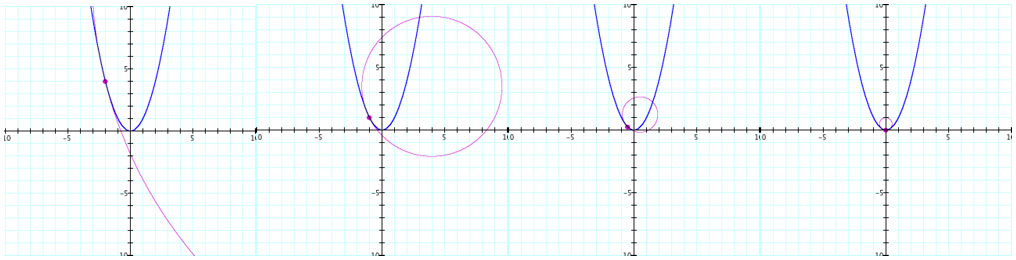
\includegraphics[height=0.2\textheight]{findig-crunch-spots-img/Fig 23.png}
    \caption{Caption}
    \label{fig:fig23}
    \vspace{4ex}
  \end{minipage} % end 
  \begin{minipage}[b]{\linewidth}
    \centering
    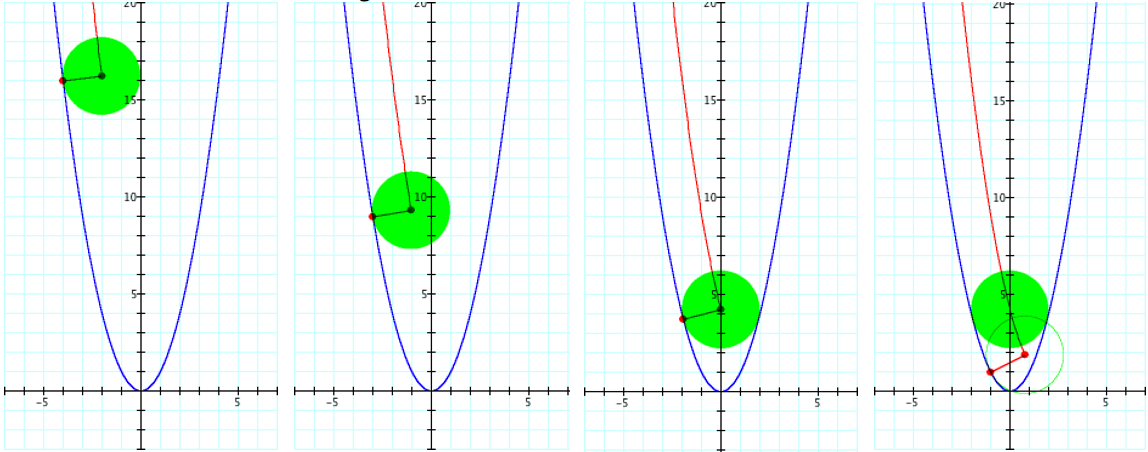
\includegraphics[height=0.2\textheight]{findig-crunch-spots-img/Fig 24.png}
    \caption{Caption}
    \label{fig:fig24}
    % \vspace{4ex}
  \end{minipage} % end
\end{figure}

Case 1, some value $x_o \in (x_1, x_2)$ gives a point $(x_o, f(x_o))$ which occurs inside the green area of the marble. This is a contradiction, as the marble cannot have rolled so far that part of the function it was rolling on is now jammed inside of it. It surely would have gotten stuck the moment it first made contact with two points of the function.

Case 2, every value $x_o \in (x_1, x_2)$ is such that $(x_o, f(x_o))$ lies exactly on the bottom edge of the circle. This means that on that interval the function is precisely a circular arc with the same radius as the marble. Immediately before and after interval $(x_1, x_2)$ the marble will have no trouble rolling along the function. During interval $(x_1, x_2$ it will rest snuggly in that little circular arc immobile. We see that no divot triangle or strange exotic behavior occurs. Note that this is a region whereon the radius of curvature is precisely $N$. This scenario is diagrammed in Figure 25 with specially constructed branching function:

\begin{equation*}
    y = 
    \begin{cases}
        \sqrt{3} \left( x - \dfrac{\sqrt{3}}{2}\right) + \dfrac{1}{2}, 
        & x \in \left( -\infty, - \dfrac{\sqrt{3}}{2} \right]
        \\
        - \sqrt{1 - x^2} + 1
        & x \in \left( - \dfrac{\sqrt{3}}{2}, \dfrac{\sqrt{3}}{2} \right)
        \\
        - \sqrt{3} \left( x + \dfrac{\sqrt{3}}{2} \right) + \dfrac{1}{2}
        & x \in \left[ \dfrac{\sqrt{3}}{2}, \infty \right)
    \end{cases}
\end{equation*}

Case 3, at least some value $x_o \in (x_1, x_2)$ gives a point $(x_o, f(x_o))$ which occurs below the
marble and does make contact with it (Fig $\ref{fig:fig26}$). For any point of the function to be below the
marble, it means that the function had to both depart away from the marble and then return back to it at some
$x_3 < x_4$ both $\in [x_1, x_2]$. Consider the tangent lines to the function $y = f(x)$ at $x_3 \land x_4$ (Fig $\ref{fig:fig27}$). They travel \textit{closer} to one another, thus meaning that the function $y = f(x)$ must at some point on $(x_3, x_4)$ take an even sharper turn than the bottom circular edge of the marble. This guarantees that somewhere on $(x_1, x_2)$ the function’s radius of curvature is less than $N$.

\begin{figure}[h!]
  \centering    
  \label{}
  \begin{minipage}[b]{0.23\linewidth}
      \centering
      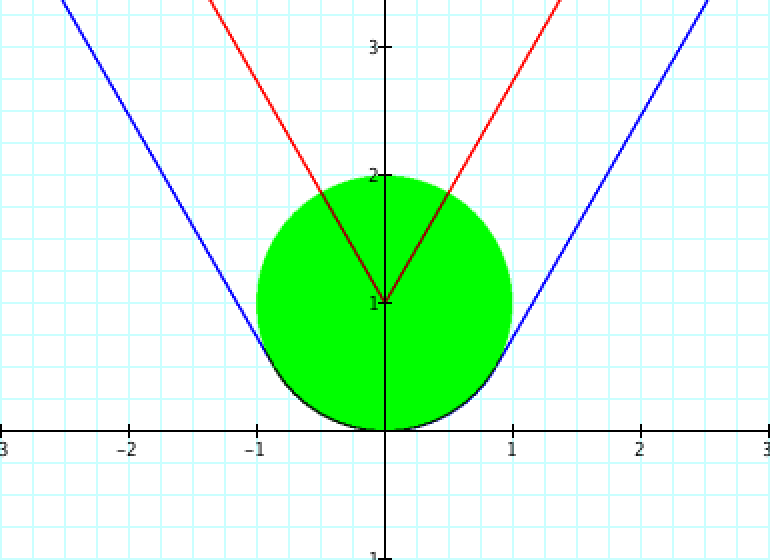
\includegraphics[width=.9\linewidth]{findig-crunch-spots-img/Fig 25.png}
      \caption{Caption}
      \label{fig:fig25}
  \end{minipage}
  \begin{minipage}[b]{0.23\linewidth}
      \centering
      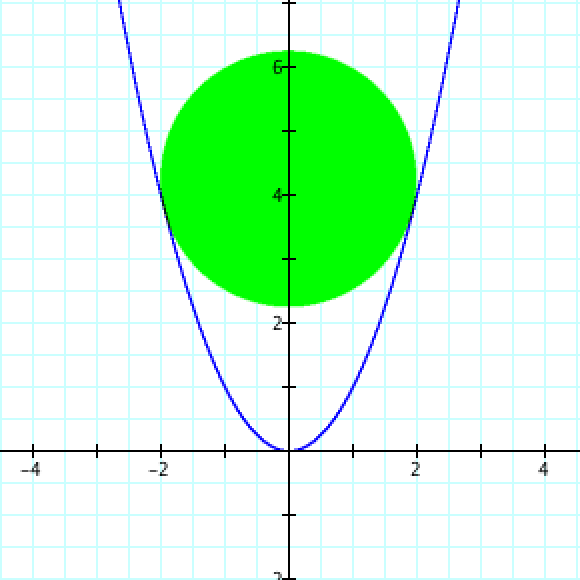
\includegraphics[width=.9\linewidth]{findig-crunch-spots-img/Fig 26.png}
      \caption{Caption}
      \label{fig:fig26}
  \end{minipage}
  \begin{minipage}[b]{0.23\linewidth}
      \centering
      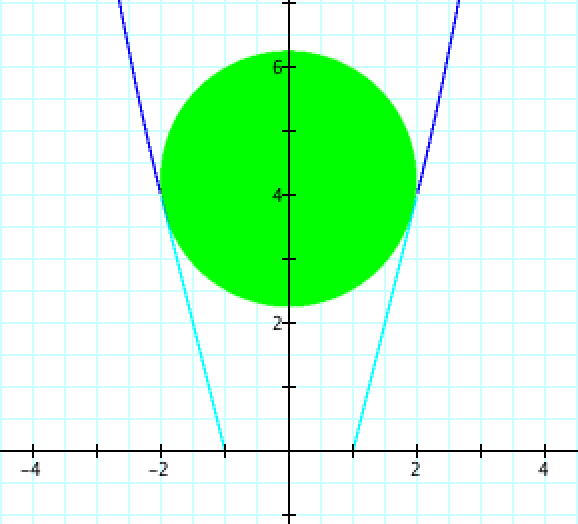
\includegraphics[width=.9\linewidth]{findig-crunch-spots-img/Fig 27.png}
      \caption{Caption}
      \label{fig:fig27}
  \end{minipage}
  \begin{minipage}[b]{0.23\linewidth}
      \centering
      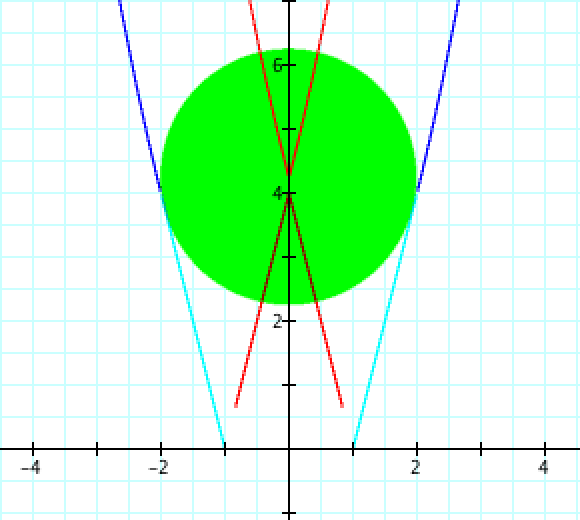
\includegraphics[width=.9\linewidth]{findig-crunch-spots-img/Fig 28.png}
      \caption{Caption}
      \label{fig:fig28}
  \end{minipage}
\end{figure}

Extending those tangent lines shows that immediately after $x_3$ the left tangent line (which $f(x)$ approximates, even if only briefly) spawns an $N$-Units Away point which is to the \textit{right} of the center point of the marble (Fig $\ref{fig:fig28}$). Likewise just before $x_4$ the right tangent line (which $f(x)$ approximates) spawns an $N$-Units Away point which is to the left of the center point of the marble. Both of these points are also \textit{below} the centerpoint thus guaranteeing that the N-Units Away Curve will now fail the Vertical Line Test and we are seeing a budding divot triangle, occurring \textit{below} the Snipped N-Units Away Curve.

When you are rolling a marble of radius $N$ towards an interval of the function with radius of curvature less than $N$, we will always find a divot triangle.

But it works the other way around too. If you ever find a divot triangle on an $N$-Units Away Curve, then precisely at the apex of the triangle a marble of radius $N$ would have gotten stuck. The light blue tangent lines continue towards one another getting \textit{closer}, thus necessarily meaning that the function $y = f(x)$ took a sharper turn than the bottom circular edge of the marble. Like before, this guarantees that somewhere on $(x_3, x_4)$ the function had radius of curvature less than $N$.

Thus, $f(x)$ achieves a radius of curvature $ < N \iff $ a divot triangle is present.

This lets us precisely locate where all of the divot triangles first appear! The $N$-Units Away Curve for $y = f(x)$ will ``crunch'' upon itself and spawn a divot triangle at exactly those values of $x$ which gives local minimums of the radius of curvature of $f(x)$. Furthermore the critical value of $N$ which causes the crunching phenomenon to occur will be precisely the value of that local minimum of the radius of curvature.

All of the above was thought out with the assumption that $N$ is positive. If $N$ is negative, you have a marble rolling along the ``ceiling'' curve of a function with reversed gravity pointing upwards. Marbles can only get stuck when the function curves \textit{towards} them. Thus crunch spots above the function will be created when the function is concave up aka when $f''$ is positive and crunch spots below the function will be created when the function is concave down aka when $f''$ is negative.

We now summarize all of these findings into one big theorem:

\begin{myTrm}

    A twice differentiable function $f(x)$ whose second derivative is continuous produces a unique crunch spot of its $N$-Units Away Curves at precisely the values of $x$ which give the radius of curvature function $R(x)$ a local minimum. The crunch spot of $\mathbb{R}^2$ associated with each minimum $x_m$ is found exactly $R(x_m)$ units along the normal line to the function $y=f(x)$ at $x=x_m$ in the direction up or down corresponding to the sign of $f''$. . This location can be found by plugging $t_m = x_m$ into the equation for the $\left( \dfrac{f''(t_n)}{|f''(t_n)|} R(t_n) \right)$-Units Away Curve.

\end{myTrm}

\subsection{An example}

Let us now do an example to show the true power of this theorem.

Take as our function a classic: $y = x^3$. Where are its crunch spots to be located? Plot the function $y = x^3$ and now also plot its radius of curvature function: $R(x) = \dfrac{(1 + f'(x))^2)^{3/2}}{|f''(x)|}$. Figure $\ref{fig:fig9-29}$ displays both of these. Using computerized approximation, we see that $R(x)$ has two local minimums, one at $(-0.386, 0.567)$ the other at $(0.386, 0.567)$... (Fig $\ref{fig:fig9-30}$.

The previous theorem tells us that we should be able to find the first of the two crunch spots on $\mathbb{R}^2$ by plugging $t_{m_1} = -0.386$ and $N = \dfrac{f''(t_{m_1})}{|f''(t_{m_1})|} 0.567 = -0.567$ into Formula 2 for the $N$-Units Away Curve: $ f_N(t) = \begin{bmatrix} t - N f'(t) ((f'(t))^2 + 1)^{-1/2} \\ f(t) + N ((f'(t))^2 + 1)^{-1/2} \end{bmatrix} $.

$$\implies f_{-0.567}(-0.366) = \begin{bmatrix}
-0.366 + 0.567 f'(-0.366) ((f'(-0.366))^2 + 1)^{-1/2} \\ f(-0.366) -0.567 ((f'(-0.366))^2 + 1)^{-1/2}
\end{bmatrix} = \begin{bmatrix} -0.155 \\ -0.575 \end{bmatrix}$$

Doing the same with $t_{m_2} = 0.366$ and N = $\dfrac{f''(t_{m_2})}{|f''(t_{m_2})|} 0.567 = 0.567$ gives:

$$\implies f_{0.567}(0.366) = \begin{bmatrix}0.366 - 0.567 f'(0.366) ((f'(0.366))^2 + 1)^{-1/2} \\ f(0.366) + 0.567 ((f'(0.366))^2 + 1)^{-1/2}
\end{bmatrix} = \begin{bmatrix} 0.155 \\ 0.575 \end{bmatrix}$$.

These two points are plotted net to $y = x^3$ in figure $\ref{fig:fig9-31}$. Are these the crunch spots?

Figure $\ref{fig:fig9-32}$ shows that indeed these two points are none other than exactly the two crunch spots for $y = x^3$.

\begin{figure}[H] %{l}{0.3\linewidth}
    \begin{minipage}[b]{0.2\linewidth}
        \centering
        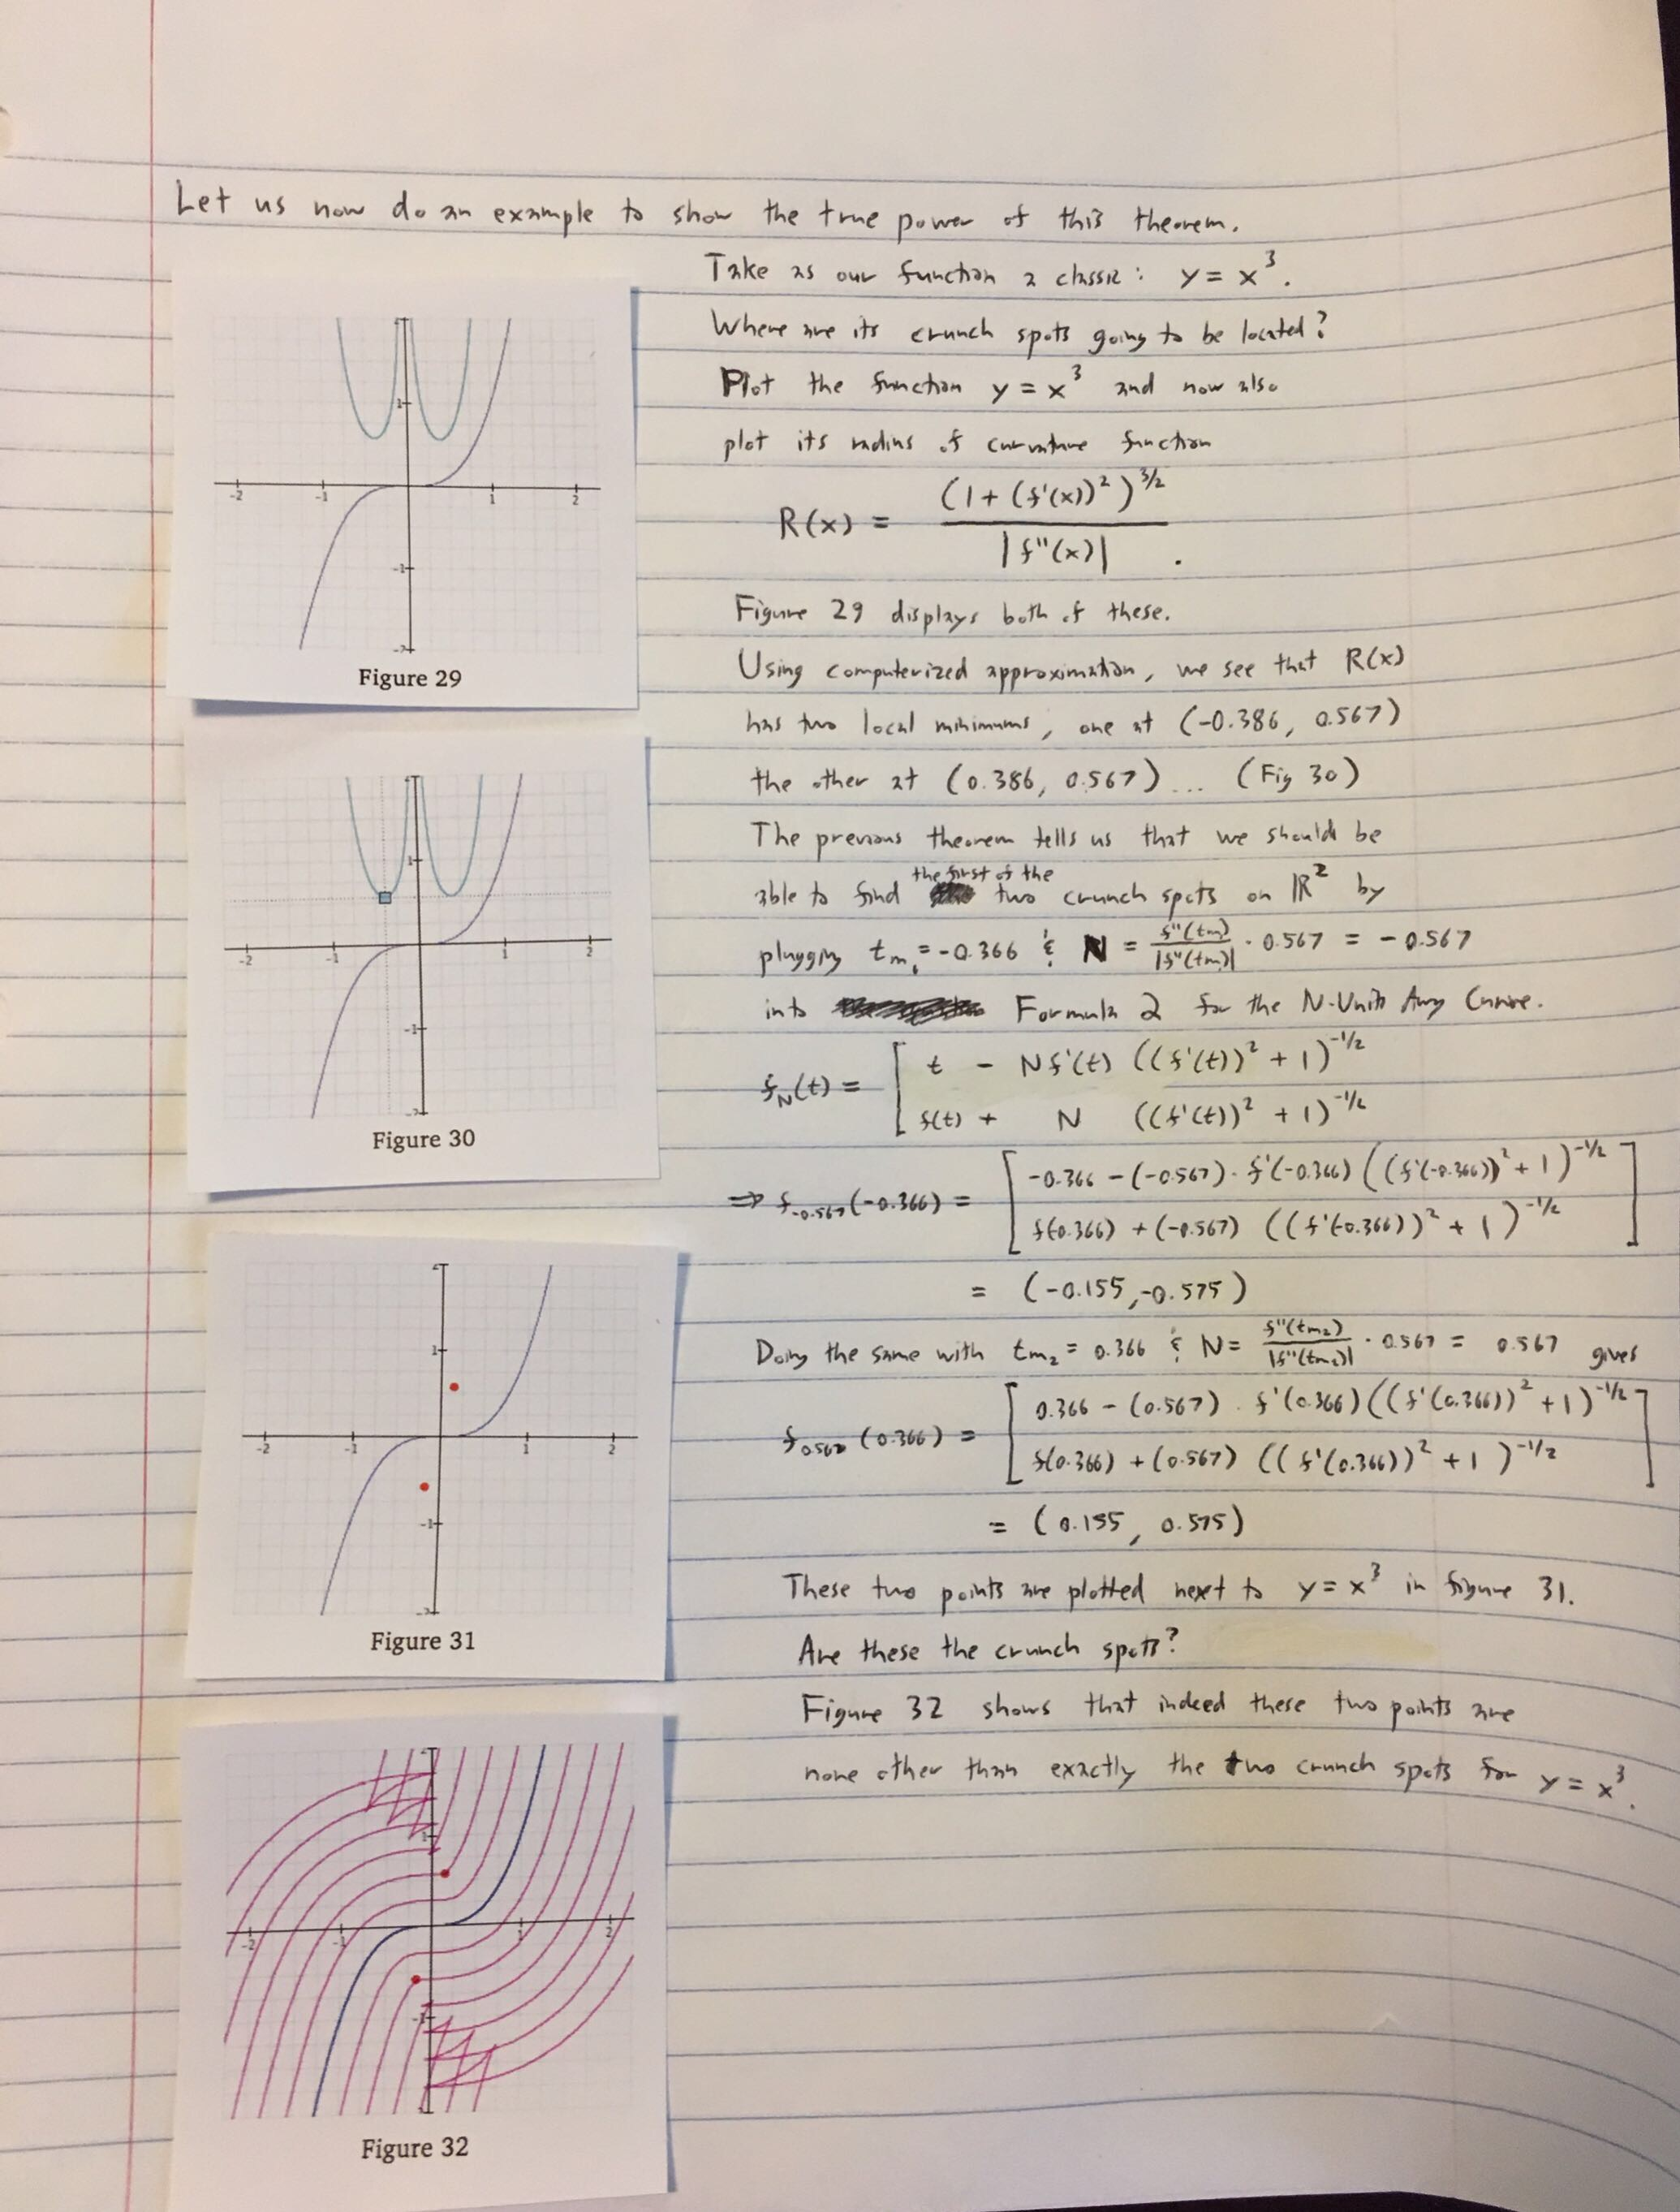
\includegraphics[height=0.1\textheight]{findig-crunch-spots-img/Fig 9-29.png}
        \caption{Caption}
        \label{fig:fig9-29}
    \end{minipage}
    \begin{minipage}[b]{0.2\linewidth}
        \centering
        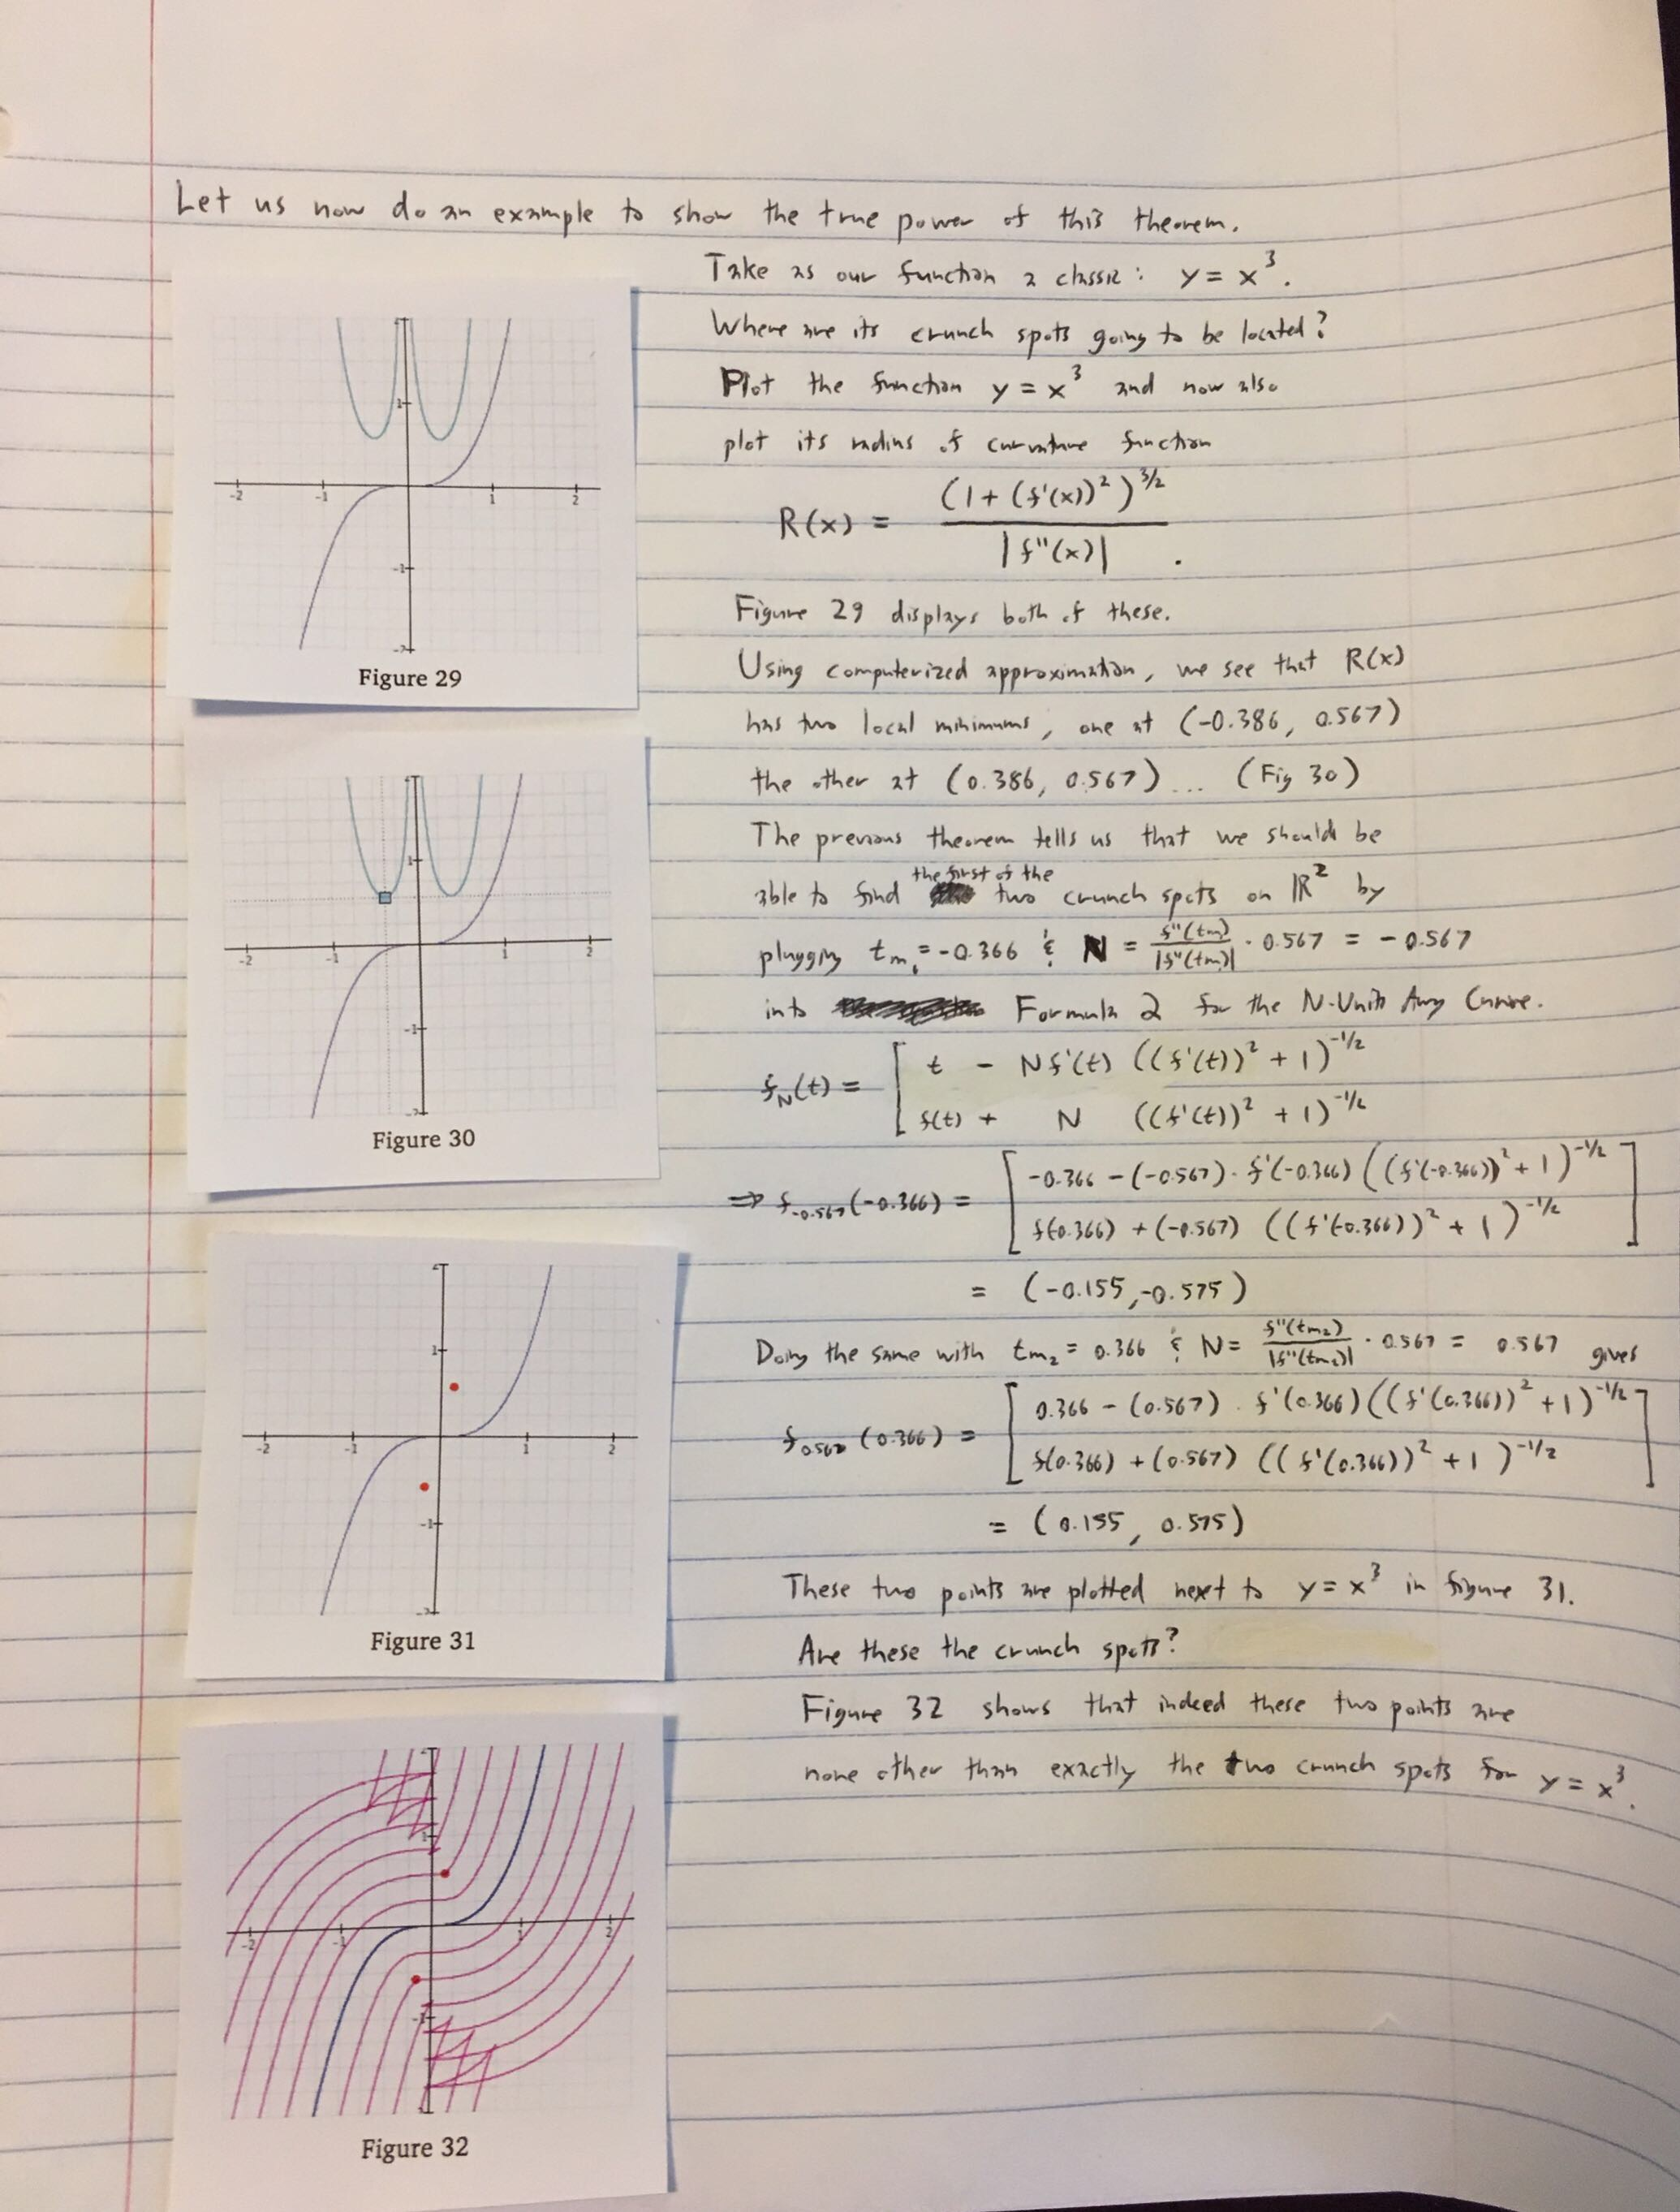
\includegraphics[height=0.1\textheight]{findig-crunch-spots-img/Fig 9-30.png}
        \caption{Caption}
        \label{fig:fig9-30}
    \end{minipage}
    \begin{minipage}[b]{0.2\linewidth}
        \centering
        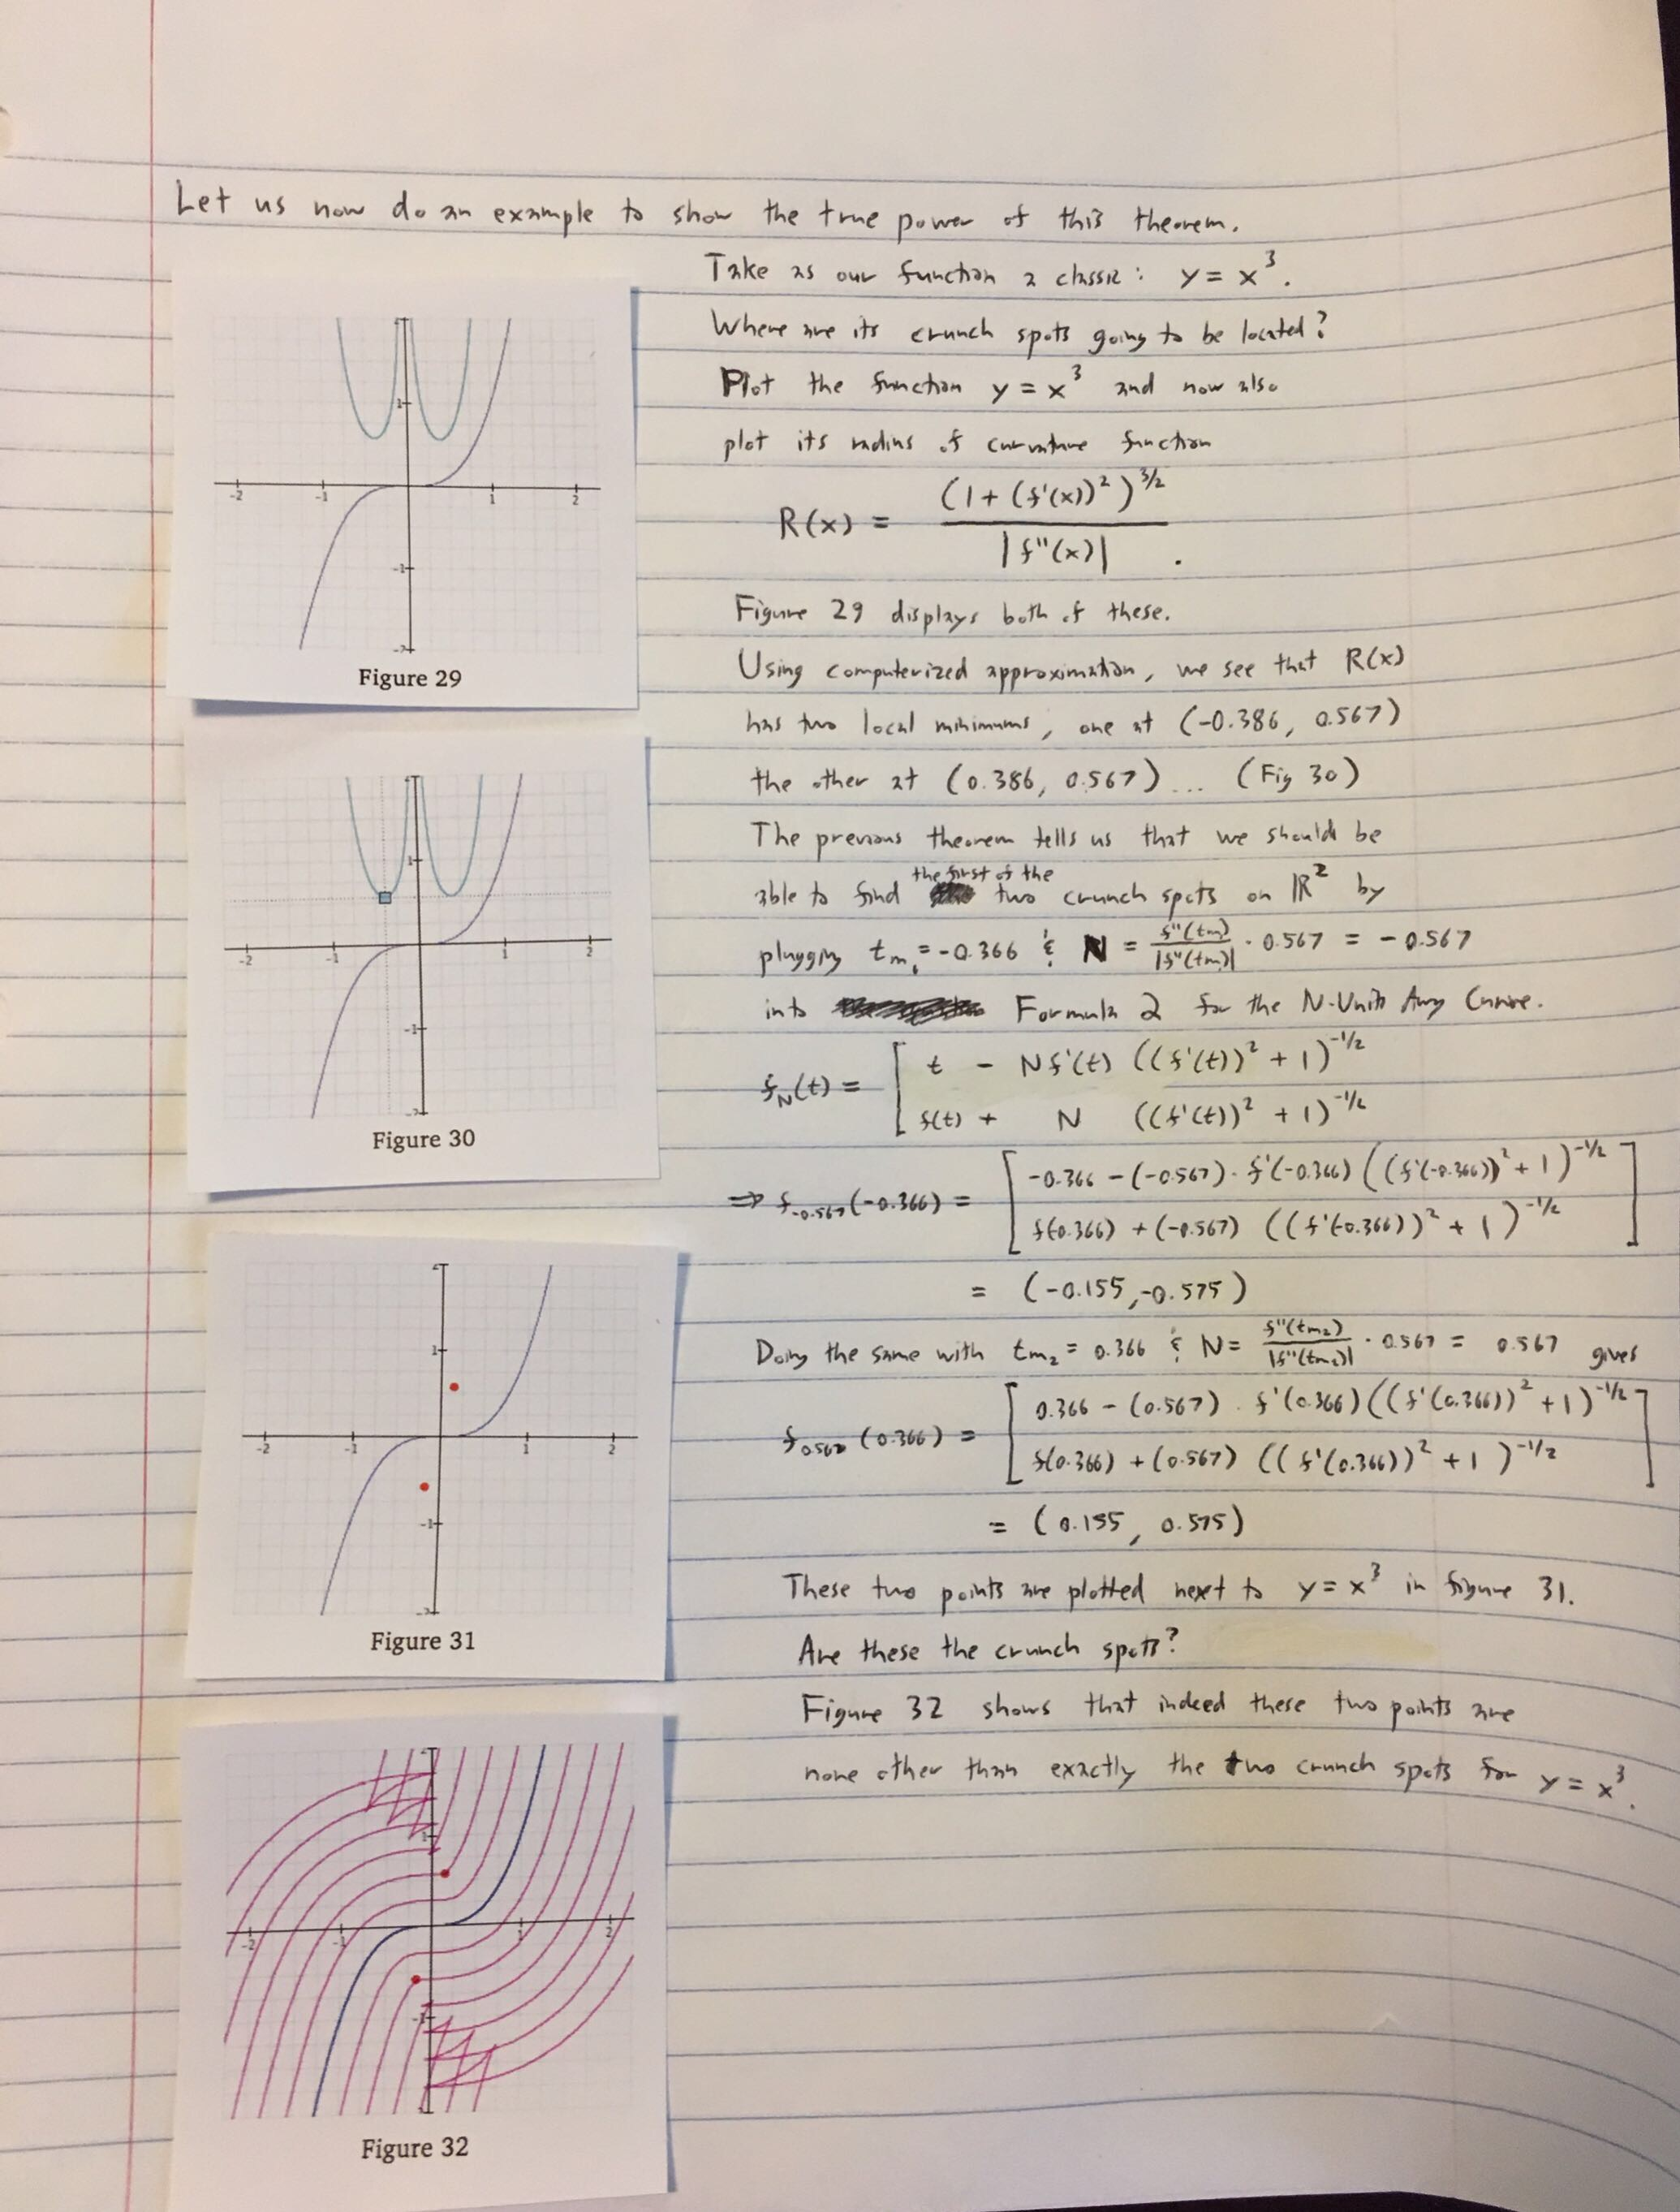
\includegraphics[height=0.1\textheight]{findig-crunch-spots-img/Fig 9-31.png}
        \caption{Caption}
        \label{fig:fig9-31}
    \end{minipage}
    \begin{minipage}[b]{0.2\linewidth}
        \centering
        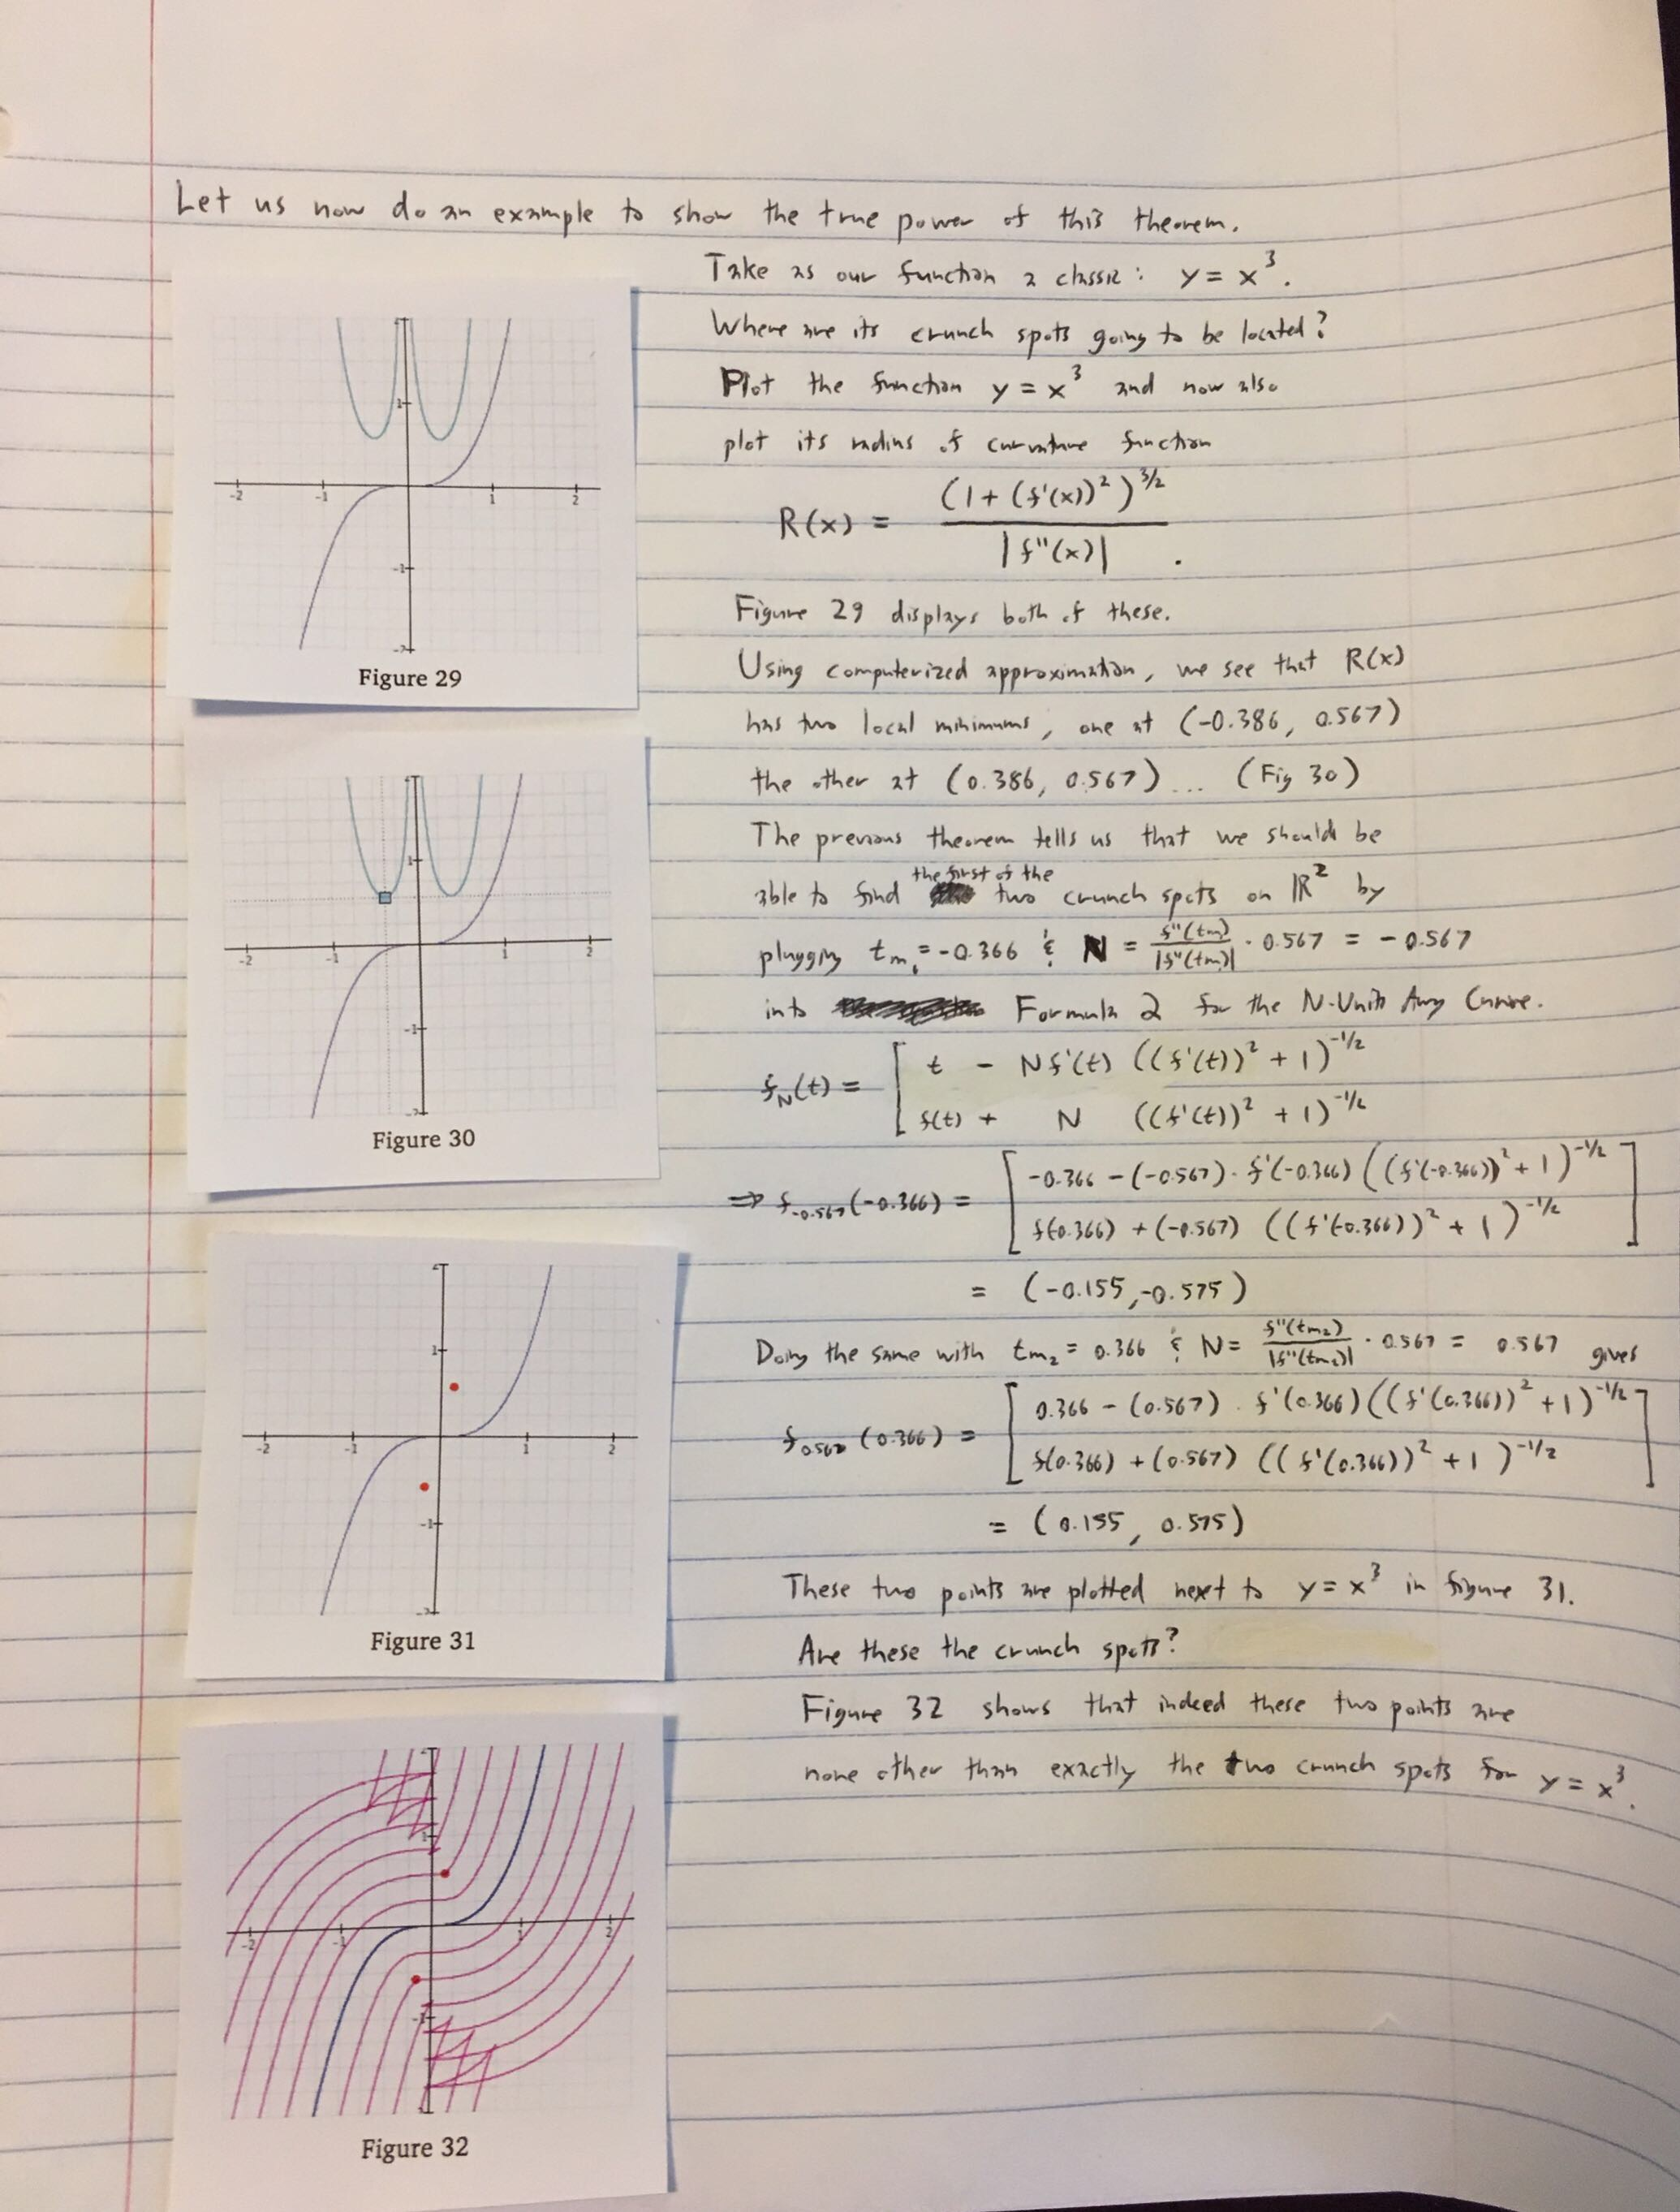
\includegraphics[height=0.1\textheight]{findig-crunch-spots-img/Fig 9-32.png}
        \caption{Caption}
        \label{fig:fig9-32}
    \end{minipage}
\end{figure}